% SAFA --- IEEE Open Journal template (IEEE-open-journal-template.zip: ieeetj.cls,
% tj-template-s1.tex conventions). English version of sn-article.tex.
% Terminology follows GLOSSARY.md — keep the two versions consistent.
% ieeetj.cls is included in the repo (identical to the zip). Uppercase section
% titles, \IEEEPARstart, and front matter follow the template conventions.
\documentclass{ieeetj}

\usepackage{graphicx}
\usepackage{amsmath,amssymb,amsfonts}
\newcommand{\cmark}{\ensuremath{\checkmark}}   % table: public
\newcommand{\xmark}{\ensuremath{\times}}        % table: closed/none
\usepackage{amsthm}
\usepackage{mathrsfs}
\usepackage{booktabs}
\usepackage{multirow}
\usepackage{xcolor}
\usepackage{algorithm}
\usepackage{algpseudocode}
\usepackage{algcompatible}   % uppercase macros \STATE \IF \FOR etc. (Algorithm 1)
\providecommand{\RETURN}{\State \Return}  % some TeXLive algcompatible lacks \RETURN -> supply (ignored if defined)
\usepackage{cite}
\usepackage{placeins}         % \FloatBarrier — keep figures inside section/bibliography boundaries
\usepackage{subcaption}       % 2x2 concept diagram (subfigures)
\usepackage[hidelinks]{hyperref}
\usepackage{orcidlink}       % author ORCID icons (\orcidlink)
\AtBeginDocument{\definecolor{tmlcncolor}{cmyk}{0.93,0.59,0.15,0.02}\definecolor{NavyBlue}{RGB}{0,86,125}}
\def\OJlogo{\vspace{-4pt}}
\def\seclogo{\vspace{10pt}}
\def\authorrefmark#1{\ensuremath{^{\textbf{#1}}}}

\newtheorem{theorem}{Theorem}
\newtheorem{proposition}[theorem]{Proposition}
\newtheorem{definition}{Definition}
\newtheorem{remark}{Remark}

\begin{document}

\receiveddate{XX Month, XXXX}
\reviseddate{XX Month, XXXX}
\accepteddate{XX Month, XXXX}
\publisheddate{XX Month, XXXX}
\currentdate{XX Month, XXXX}
\doiinfo{XXXX.XXXX.0000000}

\markboth{SAFA: Keeping the Efficiency--Fairness Balance with Lightweight, Queue-Only Reordering}{Cho \MakeLowercase{et al.}}

\title{SAFA: Keeping the Efficiency--Fairness Balance with Lightweight, Queue-Only Reordering}

\author{Kyunam~Cho\authorrefmark{1}\authorrefmark{2}\,\orcidlink{0000-0002-8300-8192}, YoungHwan~Jin\authorrefmark{2}, and Heonchang~Yu\authorrefmark{1}\,\orcidlink{0000-0003-2216-595X}}
\affil{Department of Computer Science and Engineering, Korea University, Seoul, Republic of Korea}
\affil{LG Uplus Corp., Seoul, Republic of Korea}
\corresp{Corresponding author: Heonchang Yu (e-mail: yuhc@korea.ac.kr).}
\authornote{K. Cho e-mail: mystous@korea.ac.kr. Y. Jin e-mail: yhjin@korea.ac.kr.}

\begin{abstract}
Deep-learning training jobs in datacenters can run only after securing multiple GPUs simultaneously. As jobs with widely varying GPU demands are allocated repeatedly, unallocated GPUs become scattered across nodes, and even when the cluster-wide unallocated total is sufficient, no single server has enough GPUs for a large job. As a result, once the large job at the head of the queue cannot be placed (HOL, Head-of-Line blocking), the jobs behind it are blocked as well, and starvation occurs. A scheduler operates in two stages: which job to serve first (Order) and where to place it (Placement). This work presents SAFA (Starvation-Aware Fair Aging), which focuses on the first stage, Order. As a pre-placement reordering layer that handles Order only, SAFA reorders the queue using only signals directly observable in the queue---each job's waiting time, resource demand, and relative age---so that the system as a whole can be used efficiently. SAFA's reordering moderates the efficiency loss that comes with resolving HOL, suppressing the trade-off and preserving the balance. Rather than being pre-computed as a workload-specific value, the coefficient controlling this trade-off is computed dynamically from queue statistics, so no re-tuning is needed even in training environments where the job mix changes constantly. To validate SAFA's performance, we compared it against the non-intervening baseline FIFO and six Order policies (SJF, LAS, Kueue, EASY, Themis, Lucid) on a discrete-event simulator (256--1024 GPUs, single cluster). Using the 111k-job Philly trace, the experiments show that in deeply contended overload configurations, while the bottom-1\% order fairness of all six policies collapses to 0, SAFA alone keeps it at 92--95 while reducing the queue wait by 7--13\% relative to FIFO and raising average GPU utilization from 92\% to 95--96\%. The same trend was reproduced on two additional independent large-scale traces (Helios, Alibaba), and the starvation-prevention behavior was verified through real-cluster measurements on an NVIDIA B200$\times$8 single-node Kubernetes cluster. SAFA also composes with seven Placement policies (most-allocated, compact, round-robin, MCTS, FGD, KAI binpack, KAI spread), and when combined with KAI and FGD it raised the allocation rate by 4--5.8\%p.
\end{abstract}

\begin{IEEEkeywords}
Head-of-line blocking, GPU gang scheduling, queue reordering, order fairness, tuning-free (zero-knob) scheduling, placement-agnostic reordering layer, datacenter GPU.
\end{IEEEkeywords}

\maketitle

\section{INTRODUCTION}\label{sec1}
\IEEEPARstart{J}{ob} scheduling for GPU clusters has long been studied as a key problem that governs operating and research costs. Large organizations build ``hyper-clusters'' that tie hundreds to thousands of GPUs together with high-bandwidth interconnects, and as jobs with disparate GPU request counts and JCTs are submitted endlessly, resources become fragmented\cite{athlur2022varuna}. Fragmentation grows even more severe in shared environments that use fractional GPUs: hundreds of GPUs may sit idle cluster-wide yet cannot be assigned to new jobs\cite{weng2023beware}. Nor can scheduling fully solve this, because queue assignment of jobs whose completion times cannot be known in advance is NP-hard combinatorial optimization\cite{ullman1975np}, and real scheduling maps onto flow shop, job shop, single machine, open shop, and $k$-machine parallel scheduling\cite{b1}, so approximation algorithms are usually relied upon\cite{b2}.

Despite these difficulties, scheduler research for deep-learning jobs has advanced steadily. Ye et al.\cite{b3} organize the field along two axes: one classifies by workload type, such as training or inference, and the other by objective, such as efficiency, fairness, and deadlines. They single out Sia\cite{b4}, which leads across utilization, fairness, and completion time, and Lucid\cite{b5}, which boosts performance with multi-state profiling, as representative SOTA schedulers, and view most of today's GPU schedulers as variants of this lineage. These schedulers, however, share one common burden: whenever workload characteristics change, the policy or the scheduler must be re-fit.

In addition, recently proposed GPU schedulers each carry further limitations of their own. For the learning-to-rank-based LLM scheduler of Fu et al.\cite{fu2024efficient}, the ranking metric Kendall's Tau has been reported to poorly reflect end-to-end performance, and its fit with recent LLM-serving optimizations remains insufficiently validated\cite{fu2024efficient}. Fragmentation Gradient Descent (FGD)\cite{weng2023beware} measures fragmentation only within a narrow ``one-step'' scope to preserve scheduler independence, which can yield suboptimal choices in early phases when resources are still plentiful. Elastic schedulers such as Optimus\cite{peng2018optimus} estimate training speed and convergence with online performance models, but they are sensitive to prediction error (up to 20\% in convergence estimation) and pay checkpoint overhead at every resource reconfiguration. Themis\cite{mahajan2020themis} pursues fairness and placement sensitivity at once, at the cost of a central solver-based round auction and complex app-submitted inputs (detailed in \S\ref{Related}).

Such sophisticated schedulers commonly depend on information outside the queue---ranking models, performance/throughput profiles, runtime estimates, auction-solver inputs, and so on---and such auxiliary information entails profiling cost, prediction error, and computational overhead, and requires dedicated infrastructure. This work proposes Starvation-Aware Fair Aging (SAFA), which remedies these drawbacks. SAFA operates only on information directly observable in the queue (waiting time, resource demand, relative age). It does not attack the NP-hard problem head-on; it removes only the Head-of-Line blocking (HOL)\cite{karol1987hol}---the classic packet-switching problem in which a blocked head job delays the jobs behind it, and which also arises structurally in GPU server pools---that stems from resource fragmentation. Leaving the core scheduler untouched, it mitigates the queue delay and arrival-order unfairness that HOL causes. SAFA's key contributions are as follows.
\begin{enumerate}
\item Starvation-free reordering: A large job requesting close to a single server's maximum GPU count sometimes fails to obtain a gang-scheduling slot and starves, and once the queue head is blocked (HOL), subsequent jobs are delayed even while GPUs remain available. SAFA monitors pending jobs' waiting times and resource demands and reorders the queue dynamically, mitigating HOL-induced queue delay while preserving arrival-order fairness. Because reordering weighs each job's accumulated age together with its fitness for vacant slots, large jobs are not unconditionally excluded---subsequent jobs that fit the vacant slots are advanced, while a large job also accumulates age as it waits, raising its priority relative to the rest.
\item Placement composability: SAFA decides Order only (which job first) and does not touch Placement (where to place), so it can be attached, as is, in front of diverse Placement policies without replacing the core scheduler. This composability holds across all seven Placement policies (most-allocated, compact, round-robin, MCTS, FGD, KAI binpack, KAI spread), and the more fragmentation-prone (scattering) the placement, the larger the recovery of HOL-wasted resources.
\item Tuning-free coefficient (Zero-knob): The trade-off between removing HOL and preserving fairness is governed by the coefficient $\alpha$; since $\alpha$ is normalized by observed queue-age statistics and resource fitness and determined dynamically, the tuning knob is eliminated and no re-tuning is needed as the workload changes.

\end{enumerate}

The rest of this paper is organized as follows. Section \ref{Related} reviews related work; Section \ref{motivation} establishes the need for queue adjustment; Section \ref{algo:intro} presents the mathematical details of queue adjustment and tuning-free balance keeping; Section \ref{sec:eval} evaluates on public traces (Philly, Helios, Alibaba) and with real B200 Kubernetes measurements; Section \ref{conclu} gives a summary and future directions.

Throughout this paper, `GPU' refers to a datacenter GPU. The precise term is `datacenter GPU', shortened for brevity.

\section{RELATED WORKS}\label{Related}
To compare SAFA fairly, this work distinguishes prior studies along two aspects. The first aspect is the stage at which a scheduler intervenes. Scheduling stages can be divided in many ways, but broadly into an Order stage that decides which job to serve first and a Placement stage that decides where to put the selected job. The second aspect is what information the decision uses: does it operate only on information directly observable in the queue---waiting time, resource demand, queue position, and observed cumulative usage---or does it rely on auxiliary information beyond that? Auxiliary information splits into three kinds---first, runtime estimation or rank prediction (SJF, EASY backfilling, learning-to-rank); second, per-job performance/throughput profiles (Optimus, Lucid, Sia, Pollux, Arena, Rubick); third, round solvers or auction bids (Themis, FFT, RLTune).


\begin{table*}[htb!]
\centering
\caption{Scheduler taxonomy}
\label{tab:related}
\scriptsize
\setlength{\tabcolsep}{4pt}
\begin{tabular}{@{}lllcl@{}}
\toprule
\textbf{System} & \textbf{Venue} & \textbf{Decision axis (information assumption)} & \textbf{Exp.} & \textbf{Rationale / representative baseline} \\
\midrule
\multicolumn{5}{@{}l}{\textit{Experimental baselines --- same layer, comparable information}}\\
FIFO / gate-FIFO & --- & queue order (none) & $\checkmark$ & control (pure policy effect)\\
SJF & classic & queue order (duration) & $\checkmark$ & mean-optimal reference\\
LAS (Tiresias)\cite{gu2019tiresias} & NSDI'19 & queue order (attained service) & $\checkmark$ & least-attained\\
Kueue\cite{kueue2024} & k8s & quota gate & $\checkmark$ & production standard\\
EASY\cite{mualem2001backfilling} & HPC & reservation+backfill (duration estimates) & $\checkmark$ & perfect-estimate variant (not an upper bound)\\
Themis\cite{mahajan2020themis} & NSDI'20 & round auction (finish-time-fair) & $\checkmark$ & fairness/solver axis\\
Lucid\cite{b5} & ASPLOS'23 & profile packing & $\checkmark$(adapted) & \shortstack[l]{synthetic util, duration-oracle injection ---\\single scalar bounds synthesis distortion}\\
\textbf{SAFA (Zero-knob)} & --- & queue order (age, zero prediction) & $\checkmark$ & this work (information-free)\\
\midrule
\multicolumn{5}{@{}l}{\textit{Orthogonal Placement axis --- for invariance validation, not Order comparators}}\\
FGD\cite{weng2023beware} & ATC'23 & Placement (fragmentation avoidance) & $\checkmark$ & Placement axis (prototype); indiscriminative under oversaturation\\
KAI\cite{kai2025} & k8s & Placement (binpack/spread) & $\checkmark$ & Placement axis (production); SAFA$\oplus$KAI composition\\
\midrule
\multicolumn{5}{@{}l}{\textit{Related work --- decision variables absent from traces (or layer mismatch)}}\\
Learning-to-Rank\cite{fu2024efficient} & NeurIPS'24 & LLM request order (ms) & --- & layer mismatch; represented by SJF\\
NotebookOS\cite{notebookos2026} & ASPLOS'26 & interactive replication & --- & different workload (out of scope)\\
Sia\cite{b4} & SOSP'23 & elastic ILP (goodput profiles) & --- & profile decision variables absent from traces\\
Optimus\cite{peng2018optimus} & EuroSys'18 & elastic worker/PS (performance model) & --- & performance-model decision variables absent\\
Pollux\cite{qiao2021pollux} & OSDI'21 & elastic goodput (profiles) & --- & goodput profiles absent\\
Arena\cite{arena2026} & EuroSys'26 & adaptive parallelization (profiles+estimates) & --- & execution-plan decision variables absent\\
Rubick\cite{rubick2025} & MLSys'25 & execution-plan reconfiguration & --- & execution-plan decision variables absent\\
RLTune\cite{rltune2025} & SoCC'25 & RL ordering+MILP (learned model) & --- & learning+solver; represented by Lucid/Themis\\
FFT\cite{fft2025} & ICS'25 & round cost-min (epoch estimates) & --- & solver+estimates; represented by Themis (FTF)\\
Tetris\cite{grandl2014multi} & SIGCOMM'14 & multi-dimensional resource alignment (order$+$placement) & --- & decision variables absent; couples Placement\\
Maui\cite{jackson2001maui} & JSSPP'01 & multi-factor priority (runtime, fairshare) & --- & relies on auxiliary information; residual aging is FIFO\\
\bottomrule
\end{tabular}
\end{table*}

\subsection{Techniques by Scheduling Stage}
We first look at the Order stage. Kueue\cite{kueue2024} is a Kubernetes-native queueing system that suspends and resumes jobs and provides quota-based fair sharing. Because it operates only at a gating layer without replacing the core scheduler, it is this paper's most direct production-standard baseline. Its fairness, however, is confined to quota distribution and does not resolve HOL starvation or fragmentation. Moreover, quota fairness itself manifests only under multi-Virtual-Cluster (VC) contention, so it degenerates to FIFO in a single VC. LAS in Tiresias\cite{gu2019tiresias} is an information-free discipline that favors jobs with the least accumulated resource usage and, combined with multi-level feedback queues and preemption, reduces mean JCT. However, because GPUs operate non-preemptively, pending jobs' accumulated resource usage becomes 0 and it degenerates to non-blocking FCFS, which may differ from its original behavior in which preemption is central. On the Placement axis there are two techniques. FGD\cite{weng2023beware}, for shared clusters heavily fragmented by partial GPU occupancy (21--42\% in traces), quantifies the probability that a random job cannot be scheduled, places jobs on the node with the smallest increase $\Delta F$ in that probability, and reduces unallocated GPUs by up to 49\% (using only queue and node occupancy, no profiles). The production scheduler KAI\cite{kai2025} provides binpack/spread; the default binpack gives higher scores ($\text{score}\propto 1-(\text{free}-\min)/(\max-\min)$) to nodes with fewer unallocated GPUs, consolidating jobs and leaving empty nodes for large gangs.

\subsection{Techniques Relying on Auxiliary Information}
Techniques relying on auxiliary information are examined in three branches, divided by what kind of information they additionally require for decision-making --- (i) runtime estimation and rank prediction, (ii) per-job performance/throughput profiles, and (iii) round solvers and auction bids. Down this list, the required information becomes increasingly costly to acquire (estimation error, profiling, dedicated infrastructure).

(i) Runtime estimation and rank prediction: EASY backfilling\cite{mualem2001backfilling} is the HPC-standard technique that reserves resources for the queue head while advancing subsequent jobs that do not disturb the reservation; it relies on runtime estimation (user estimates are commonly off by 2--10$\times$). Learning-to-Rank\cite{fu2024efficient} approximates SJF/SRTF in LLM serving using only the relative rank of output lengths, but it relies on rank prediction of future information---output length---and operates at request (iteration) granularity.

(ii) Per-job performance/throughput profiles: Lucid\cite{b5} collocates small jobs based on per-job utilization profiles to reduce mean JCT. The elastic, profile-driven Optimus\cite{peng2018optimus}, Sia\cite{b4}, Pollux\cite{qiao2021pollux}, Arena\cite{arena2026}, and Rubick\cite{rubick2025} optimize GPU count/type, batch size, or parallelization plans every round and require per-job goodput/throughput profiles; such profiling carries cost and error (up to 2.12$\times$ error in linear throughput extrapolation, 13--20\% JCT reduction when bypassing profiles, etc.\cite{schedmate2025}). NotebookOS\cite{notebookos2026} schedules on-demand replication for interactive notebooks, a workload inherently different from batch training.

(iii) Round solvers and auctions: Themis\cite{mahajan2020themis} introduces finish-time fairness $r$ (the ratio of completion time on the shared cluster versus a dedicated $1/N$ cluster) as a long-term fairness metric, and a central ARBITER minimizes the maximum $r$ via round auctions (apps bid with estimated $r$; strategy-proofness and Pareto efficiency are guaranteed). It depends, however, on solver auctions (p95 1,398\,ms under contention) and on app-submitted $r$ estimates. FFT\cite{fft2025} and RLTune\cite{rltune2025} presuppose a round cost-minimization solver ($+$epoch estimates) and learned RL priorities ($+$MILP node mapping), respectively.

\subsection{Baseline Selection Rationale}\label{baseline-rationale}
For a comparison to be meaningful, SAFA and the baselines must share (i) the same decision variables, (ii) the same layer, and (iii) comparable information and infrastructure assumptions. Since this work is a lightweight processing step that resolves starvation with no prior information (no runtime estimates, profiles, or solvers), we sort the same-engine comparators by their dependence on prior information (Table \ref{tab:related}). Accordingly, we adopt as baselines FIFO, LAS, and Kueue, which use queue information only; SJF, EASY, and Themis, which receive runtimes; and Lucid, whose per-job profile is defined by the trace (gpu\_utilization). For Themis, runtime information is injected with a random error of 20\%.

The remaining schedulers violate at least one of (i)--(iii) and are excluded from the baselines. (a) Missing decision variables: the decision variables of Sia, Gavel\cite{narayanan2020gavel}, Optimus, Pollux, Arena, and Rubick (per-job profiles, internal parallelization plans) do not exist in fixed-request gang traces (demoting Sia to rigid makes it equivalent to FIFO/SJF). (b) Layer mismatch: Learning-to-Rank (ms, request granularity) and NotebookOS (interactive replication) differ from cluster gang jobs in decision object and time scale, and the former's principle is represented by SJF, its perfect-prediction limit. (c) Learning/solver dependence: RLTune and FFT presuppose learned models and round solvers ($+$epoch estimates), placing them at a different information/infrastructure layer from SAFA, which uses no prediction. (d) Classical aging ancestors --- reliance on auxiliary information: Tetris\cite{grandl2014multi}, which couples resource fitness into ordering decisions, and Maui\cite{jackson2001maui}, which has operated multi-factor priority aging for decades, are SAFA's closest ancestors, but their distinguishing factors require auxiliary information that SAFA does not use, so they are not baselines at the same information layer. Maui's XFactor requires runtime estimates and its fairshare requires multi-VC usage history (stripping this information away leaves pure time-aging, which FIFO represents), while Tetris's multi-dimensional resource alignment requires decision variables absent from a single whole-GPU trace and couples Placement as well (in 1-D it degenerates to FIFO/packing). The distinctions from SAFA (coupling the resource fitness $R$; a queue-statistics-normalized tuning-free coefficient) are discussed in \S\ref{motivation}. KAI and FGD engage in Placement, so they are evaluated not as baselines but as composition targets for SAFA.


\section{MOTIVATION}\label{motivation}
The progress of deep learning is built on container-based\cite{b7} reproducible, shared training environments. Docker Hub\cite{b8} and Hugging Face\cite{b9} make ML frameworks, libraries, and architectures easy to share, letting researchers focus on algorithms. This abstraction, however, keeps models from accessing GPUs at a fine granularity and, paradoxically, breeds inefficiency in GPU server pools.

Because GPU access is abstracted at card granularity, containers usually occupy GPUs exclusively. Consequently, even when the hardware supports time slicing that could raise the allocation rate, it is hard to exploit flexibly during training or server-pool operation. Meanwhile, as model sizes grow, it has become common for a single job to demand multiple GPUs simultaneously. Jobs with disparate completion times and GPU demands are submitted to an operating server pool without pause, and combined with exclusive GPU occupancy this deepens the fragmentation inside the pool. How fragmentation arises can be illustrated with the following example.

\begin{figure}[htb!]
\centering
\begin{subfigure}{0.8\columnwidth}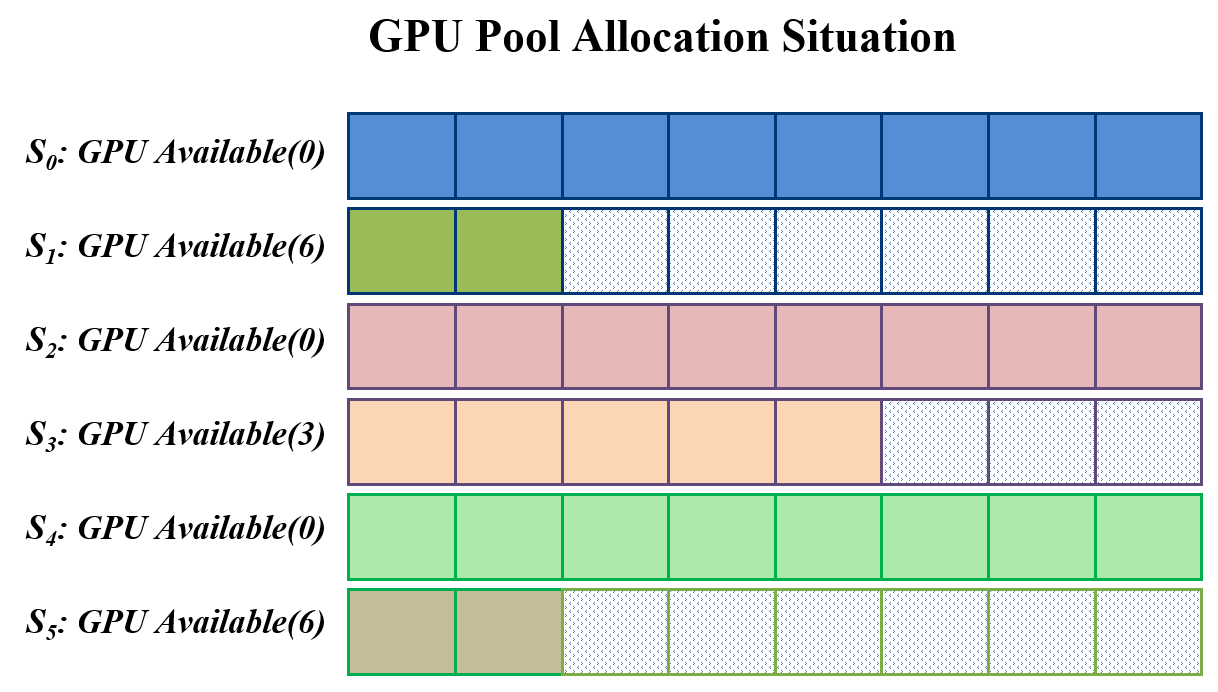
\includegraphics[width=\linewidth]{Pic/Fig_01.png}\caption{Server pool before scheduling (fragmented)}\label{fig:concept-a}\end{subfigure}

\medskip
\begin{subfigure}{0.8\columnwidth}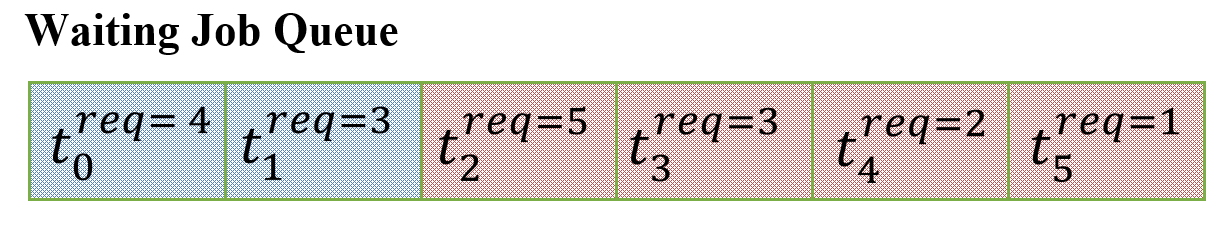
\includegraphics[width=\linewidth]{Pic/Fig_02.png}\caption{Wait queue at the same instant}\label{fig:concept-b}\end{subfigure}

\medskip
\begin{subfigure}{0.8\columnwidth}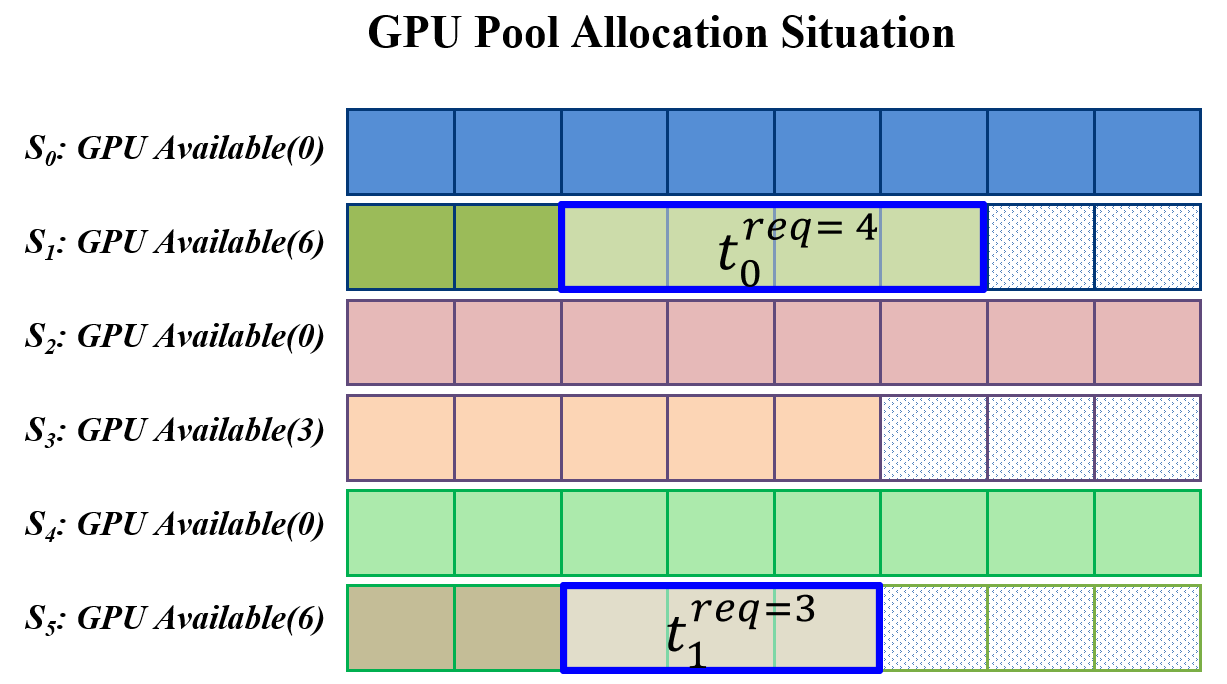
\includegraphics[width=\linewidth]{Pic/Fig_03.png}\caption{After scheduling --- HOL blocking of $t_2$}\label{fig:concept-c}\end{subfigure}

\medskip
\begin{subfigure}{0.8\columnwidth}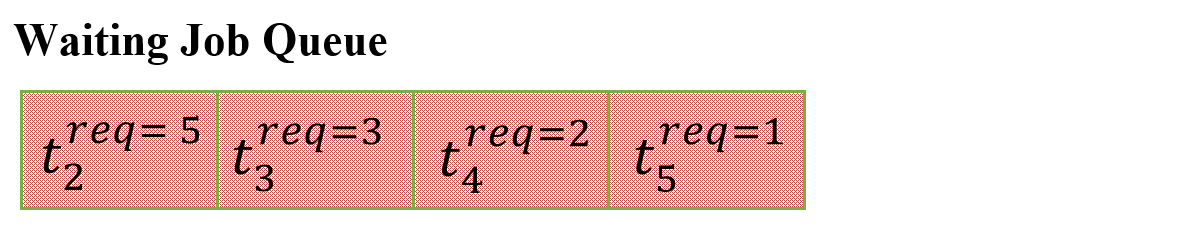
\includegraphics[width=\linewidth]{Pic/Fig_04.png}\caption{Remaining wait queue ($t_2$--$t_5$ backlog)}\label{fig:concept-d}\end{subfigure}
\caption{Fragmentation and HOL blocking}
\label{fig:concept}
\end{figure}

Figures \ref{fig:concept}(a) and (b) show the states of the GPU server pool and the job wait queue, respectively. From this state a most-allocated scheduler can allocate jobs $\textit{t}_{0}$ and $\textit{t}_{1}$. But $\textit{t}_{2}$ is in a different situation. Until other jobs complete and free up GPU slots, it cannot be scheduled because it finds no place, as in Fig. \ref{fig:concept}(c), and consequently the following $\textit{t}_{3}$, $\textit{t}_{4}$, and $\textit{t}_{5}$ can be scheduled only after $\textit{t}_{2}$ has been.

The problem is that GPU slots amounting to the total that $\textit{t}_{2}$ and $\textit{t}_{3}$ demand are already free. This is precisely HOL blocking. The cause lies in the previously allocated jobs having fragmented the GPU server pool. Such fragmentation continually arises and dissolves during operation; the worst case is when every GPU server has 7 GPUs left while the HOL-blocked job requests 8.

HOL blocking in GPU gang scheduling stems from allocation being spatial and indivisible (all-or-nothing). An 8-GPU job runs only when 8 GPUs are secured simultaneously on one server; if free GPUs are scattered 7 per server across several servers, it cannot be placed even though the total suffices. Moreover, non-preemption is the de facto standard for GPU jobs---training jobs have high checkpoint-and-reload costs, and reshaping the pool's resources is impossible or very expensive. Starvation is therefore resolved only at the moment a contiguous slot that fits the job opens.

HOL blocking motivates this work because its cost is two-sided. On one side is an efficiency cost --- while the head is blocked, GPUs that the jobs behind it could use sit idle. In our evaluation this waste amounts to about 7\%p of utilization relative to FIFO (\S\ref{sec:eval}); scaled to a hyper-cluster of hundreds to thousands of GPUs, it is equivalent to tens of GPUs or more idling at all times. On the other side is a fairness cost --- existing policies that reorder the queue to avoid HOL obtain short median waits at the price of permanently starving large jobs (bottom-1\% order fairness 0). HOL is thus a double-edged problem that costs efficiency when left alone and fairness when solved clumsily, and suppressing both costs at once is the goal of this work.

The combination of indivisibility, non-preemption, and spatial fragmentation is not new in itself. It is a long-standing basic assumption of space-shared parallel job scheduling (the JSSPP lineage\cite{feitelson1996toward}), and Maui's XFactor and wait-time weights\cite{jackson2001maui} and Slurm's age factor have operated aging in exactly that context for decades. The closest prior work coupling resource fit into job-order decisions is Tetris\cite{grandl2014multi}, which combines a multi-dimensional resource alignment score with remaining-work packing and adjusts the efficiency--fairness trade-off with an explicit knob. Two new elements distinguish this work from that classical line. First, we apply an aging-aware policy, but only to queue order---not to a Placement score as Tetris does. Second, we normalize the coefficient the policy needs with queue statistics, making it tuning-free (in contrast to the explicit weight knobs of Tetris and Maui).

The HOL problem cannot be solved by algorithms alone. Even offline scheduling of finite inputs with known processing times is NP-hard\cite{ullman1975np}, and as a non-clairvoyant online problem in which completion and arrival times are unknown, separate competitive-ratio lower bounds exist\cite{motwani1994nonclairvoyant}. Furthermore, future information (completion/arrival times) is inherently unpredictable, so approaches that try to prevent HOL by estimating it (runtime estimation, performance profiles) depend on estimation error and profiling. This work therefore presents a queue-adjustment mechanism that mitigates fragmentation-induced HOL blocking after the fact, using only information already exposed in the queue (waiting time, resource demand, relative age) instead of algorithmic improvement or future prediction.

To analyze and iteratively develop this mechanism we built our own simulator---it parses job logs, replays them under multiple policies, and composes the new methodology without touching existing mechanisms. This composability shows that queue adjustment operates independently of Placement.

\section{RESOLVING HEAD-OF-LINE BLOCKING IN THE JOB QUEUE}\label{algo:intro}
In this paper, ``gang'' denotes a fixed GPU request allocated simultaneously in an all-or-nothing manner (a rigid job in the Feitelson--Rudolph taxonomy\cite{feitelson1996toward}), distinct from Ousterhout-style gang scheduling\cite{ousterhout1982gang}, i.e., coordinated time slicing.
\subsection{Starvation-Aware Queue Adjustment}
A collapse of order fairness is starvation itself---if later arrivals keep overtaking the queue, a large job's turn never comes and it never completes. Indeed, policies that pursue only median-wait reduction obtain their low medians at the price of permanently starving large jobs (Fairness 0). Order fairness is therefore not a ``nice-to-have'' property but a production requirement that guarantees no job is excluded indefinitely. The goal of queue adjustment is not throughput improvement but to reduce the queue delay of HOL-blocked jobs while preserving arrival-order fairness as much as possible. That is, what it prevents is the state in which the queue is blocked indefinitely by one job and successors pile up forever---not a completion guarantee for an individual large job. Since arbitrary priority adjustment causes unfairness, we control that trade-off with an age-weighting coefficient.

The full adjustment procedure is Algorithm \ref{alg:adjust_wait_queue}, which proceeds in three blocks at every scheduling pass: (1) sweep the server pool and update the resource fitness $R$ per request size, (2) re-base the pending jobs' relative ages and compute each job's adjusted priority $P^*$, and (3) move the job with the largest $P^*$ to the queue head. Below we walk through each block of the algorithm and explain its meaning.

The first block (the doubly nested for loop over servers) fills in the resource fitness $R_j$ by checking, for every server $S_i$, whether a request of size $j\in\{1,\dots,M_i\}$ fits within that server's idle count $f_{S_i}$. The inner if statement checks for a shortfall: if availability suffices ($j\le f_{S_i}$), $R_j=1$ (perfect fit); otherwise it decreases by $0.1$ per unit of shortfall, taking the maximum over all servers. As a result, $R_j$ is a 0--1 index summarizing ``how well a $j$-GPU job fits the pool right now.''

The second block computes the priorities. Let $P^*$ be the adjusted priorities of jobs $t_0^*,\dots,t_n^*$. Age $A_j$ is a non-negative integer incremented by 1 at every new job submission, and the block first re-bases it into the relative age $\tilde A_j=A_j-\min_k A_k$ by subtracting the minimum age in the wait queue. The following for loop then computes each pending job's $P^*$ as:

\begin{equation}
P^*_j = P_j + \alpha\, \tilde A_j \cdot R_j
\label{eq:01}
\vspace{2pt}
\end{equation}

The first term $P_j=1/\text{base}^{\,pos_j}$ is the arrival-order (FIFO) priority: with $\text{base}=2$, $pos_j=0,1,2$ gives $1,0.5,0.25$ respectively, larger meaning higher. The second term $\alpha\,\tilde A_j R_j$ is the starvation index: it adds the product of how long a job has waited ($\tilde A_j$) and how well it fits the currently vacant slots ($R_j$), and $\alpha$ sets the speed at which it inverts the arrival-order priority. For example, for the second job in the queue ($pos_j=1$, base 0.5) to overturn the head within 6 hours ($R_j=1$, one age unit per 10 minutes), $\alpha\ge0.013889$ is required---$0.013889\times36\times1=0.5$ is added, exceeding 1.0 and overtaking the head. This example, however, is a simplification that ignores the head's own age bonus. In reality the head also receives $\alpha\,\tilde A_0 R_0$, so a true inversion occurs only when the difference between the two jobs' $\tilde A\cdot R$ products exceeds the base difference---that is, only when the slot fitness $R$ differs (with uniform $R$ there is no inversion, as confirmed by measurement).

The third block (the final if statement) finds the position $i_{\max}$ of the maximum $P^*$ and, if it is not the head ($i_{\max}\neq0$), moves only that job to the front of the queue while leaving the relative order of the remaining jobs untouched. A single pass of adjustment is thus limited to ``moving forward one job that is the most starved and fits the current slots,'' so most of the arrival order is preserved.

All three inputs ($pos_j$, $\tilde A_j$, $R_j$) are directly observable in the queue. This linear form is of the same family as Kleinrock's time-dependent priority\cite{kleinrock1976queueing}, but only the form coincides---its conservation law (premised on preemption, a single server, and steady state) does not apply to our non-preemptive, space-shared gang, oversaturated setting. SAFA's distinction lies in coupling the indivisible gang resource fitness $R$ into this classical skeleton and normalizing the coefficient with queue statistics.

\begin{algorithm}
\caption{Starvation-Aware Queue Adjustment}\label{alg:adjust_wait_queue}
\textbf{Input:} \\
\hspace*{4mm} Servers $S_i$ ($i{<}n$): accelerator count $M_i$, idle count $f_{S_i}$ \\
\hspace*{4mm} Pending jobs $t_i$ ($i{<}l_{wq}$): accelerator request $a_{t_i}$, age $A_i$ \\
\hspace*{4mm} Resource fitness $R_j$ ($j\in\{1,\ldots,8\}$, initially 0)
\begin{flushleft}
\textbf{Procedure:} Updated wait queues
\end{flushleft}
\begin{algorithmic}[1]
\STATE $R \gets 0$
\STATE {}
\FOR{ $i \gets 0$ to $n-1$}
    \FOR{$j \gets 1$ to $M_i$}
        \IF{$j > f_{S_i}$}
            \STATE $R_j \gets \max\{R_j,\ 1 - ( j - f_{S_i} ) \times 0.1\}$ \COMMENT{request $j$ exceeds availability $f_{S_i}$: decrease 0.1 per shortfall}
        \ELSE
            \STATE $R_j \gets 1$ \COMMENT{sufficient availability: perfect fit}
        \ENDIF
    \ENDFOR
\ENDFOR
\STATE {}
\STATE $\tilde A_i \gets A_i - \min_k A_k,\ \forall i$ \COMMENT{re-base relative ages}
\FOR{ $i \gets 0$ to $l_{wq}-1$}
    \STATE $P_i \gets 1/\text{base}^{\,i}$ \COMMENT{$\text{base}=2$}
    \STATE $P_i^* \gets P_i + \alpha\, \tilde A_i \cdot R_{a_{t_i}}$
\ENDFOR
\STATE {}
\STATE $(P_{i_{\max}}^*, i_{\max}) \gets \max(P^*)$
\IF{$i_{\max} \neq 0$}
    \STATE $WQ \gets [\,t_{i_{\max}},\ t_0,\ \ldots,\ t_{i_{\max}-1},\ t_{i_{\max}+1},\ \ldots,\ t_{l-1}\,]$
\ENDIF
\end{algorithmic}
\end{algorithm}

SAFA acts one step ahead of Placement and uses only the wait queue and the server pool's current allocation state, so it functions as a preprocessor that grooms the queue independently of the core scheduler (excluding schedulers that perform queue scheduling themselves or depend on cumulative metrics/context).

$P^*$ is computed per job in a single pass, so the complexity is $O(l_{wq})$ (computing $R$ is linear in the number of servers).

\subsection{Optimizing the Coefficient $\alpha$ --- from Fixed to Tuning-Free}\label{sec:coeff}
This section defines the trade-off that $\alpha$ controls and its optimum, shows that the optimal $\alpha$ varies greatly with workload so that no single optimum exists for a fixed coefficient, and then derives the dynamic coefficient $\alpha_{\text{eff}}$ (Zero-knob), which delegates coefficient determination to queue statistics.

\subsubsection{Trade-off Analysis and Metric Definitions}
A large $\alpha$ lets once-blocked jobs overtake excessively and creates new unfairness, so choosing an appropriate value requires quantifying this trade-off. We group jobs' cumulative waiting times by requested accelerator count and define the change as the accumulated distance (AD). $WT_k=\sum_{j\in C_k} w_j$ is the pre-application wait sum, $C_k$ the class requesting $k$ accelerators, and $WT'_k$ the post-application sum. The weight $1/2^{8-k}$ gives greater weight to classes with larger accelerator requests.
\begin{equation}
AD = \sum_{k=1}^8 \frac{(WT'_k - WT_k)}{2^{8-k}}
\label{eq:07}
\end{equation}

Accumulating each class's worst-wait change with the same weights gives the accumulated maximum distance (AMD):

\begin{equation}
AMD = \sum_{k=1}^8 \frac{\max\limits_{j\in C_k} w'_j \;-\; \max\limits_{j\in C_k} w_j}{2^{8-k}}
\label{eq:08}
\vspace{2pt}
\end{equation}

$w_j$ and $w'_j$ are the waiting times before and after application. These two metrics and the min--max-normalized sum (Eq. \eqref{eq:09}) are objective functions for the $\alpha$ search, not evaluation metrics; that the optimal $\alpha$ shifts with the choice of weighting and normalization further reinforces the limitation of fixed coefficients. AD captures the overall wait skew and AMD the worst wait of a specific class, so minimizing both together targets average fairness and starvation suppression at once.

$\alpha$ is searched over 0.01--1.99 (step 0.01), choosing the value that minimizes an objective function summing three min--max-normalized metrics (makespan, AD, AMD).

\begin{equation}
Obj_i^{sfa} = makespan_i^{norm} + AD_i^{norm} + AMD_i^{norm}
\label{eq:09}
\vspace{2pt}
\end{equation}

\subsubsection{Limitations of Fixed Coefficients}\label{coeff:limit}
The fundamental limitation of a fixed $\alpha$ is that its optimum is not unique. Synthesizing 1,000 jobs from each of eight distributions (normal, exponential, log-normal, gamma, beta, Weibull, uniform, Poisson) and finding the per-distribution optimal $\alpha$ minimizing \eqref{eq:09} (Table \ref{fig:motivation}), it ranges from 0.22 (gamma, Poisson) to 1.63 (log-normal). No single $\alpha$ satisfies all workloads, so a fixed $\alpha$ is merely a compromise for a particular workload, and a workload change requires redoing the grid search.

\begin{table}[htb!]
\centering
\caption{Optimal $\alpha$ by distribution}
\label{fig:motivation}
\footnotesize
\setlength{\tabcolsep}{4pt}
\resizebox{\columnwidth}{!}{%
\begin{tabular}{@{}l*{8}{c}@{}}
\toprule
Distribution & Normal & Exp. & Log-normal & Gamma & Beta & Weibull & Uniform & Poisson \\
\midrule
Optimal $\alpha$ & 0.53 & 0.44 & 1.63 & 0.22 & 0.26 & 0.55 & 0.50 & 0.22 \\
\bottomrule
\end{tabular}}
\end{table}

\subsubsection{Deriving the Dynamic Coefficient $\alpha_{\text{eff}}$ (Zero-knob)}\label{SAFA}
Instead of a fixed $\alpha$ that must be re-fit for every workload, we replace $\alpha$ in Eq. \eqref{eq:01} with $\alpha_{\text{eff}}$, computed every pass from wait-queue statistics. The wait-queue statistics derive from the relative age $\tilde A_j = A_j - \min_k A_k$ of Eq. \eqref{eq:01}: the mean $A_{\text{ref}} = \max(1,\text{mean}(\tilde A))$ representing the queue's age scale, the maximum relative age $A_{\max}=\max_k \tilde A_k$, and the fitness of the worst-fitting job $R_{\min}=\min_k R_k$. From these the coefficient is defined as:

\begin{equation}
\alpha_{\text{eff}} = \frac{g}{A_{\text{ref}}\,R_{\min}},\qquad g=\min\!\Big(1,\;\frac{A_{\max}}{A_{\text{ref}}}\Big)
\label{eq:auto-alpha}
\end{equation}
The two clamps in the formula are safeguards. The denominator's $\max(1,\cdot)$ is a floor that prevents $\alpha_{\text{eff}}$ from blowing up when the queue's age differences nearly vanish, and the $\min(1,\cdot)$ on $g$ is a cap that keeps promotion from being amplified. Whenever the queue has any age spread, $g=1$, so the effective form is $\alpha_{\text{eff}}=1/(A_{\text{ref}}R_{\min})$. The relative age $\tilde A_j$ removes the absolute offset by subtracting the minimum age and removes the scale by dividing by the mean $A_{\text{ref}}$, so $\tilde A_j/A_{\text{ref}}$ becomes a dimensionless value---``how many times older than the queue average''---independent of workload and load. As queue membership changes, ages re-base automatically through $\min_k A_k$ updates. What this normalization means becomes clear when the bonus term is unfolded into a product of two relative ratios:

\begin{equation}
\alpha_{\text{eff}}\,\tilde A_j\, R_j \;=\; \underbrace{\frac{\tilde A_j}{A_{\text{ref}}}}_{\text{age vs. queue mean}} \;\times\; \underbrace{\frac{R_j}{R_{\min}}}_{\text{fitness vs. worst fit}}
\label{eq:alphaeff-define}
\end{equation}

Promotion pressure is thus the product of the age ratio ($\tilde A_j/A_{\text{ref}}$) and the fitness ratio ($R_j/R_{\min}$), jointly reflecting age relative to the mean and fitness relative to the worst fit. The largest job---the HOL culprit ($R_{\min}$)---has low fitness and is not promoted. Since $A_{\text{ref}}$ grows with arrivals and promotion pressure saturates in proportion to $R$ differences, this is not a scheme that ``prevents starvation by age'' but one that ``prevents starvation by a combination of age-normalized slot fitness.''

Raising priority by age is not new in itself (OS priority aging, Linux CFS's vruntime equalization, Tiresias\cite{gu2019tiresias}, Slurm's multifactor age factor). What distinguishes this work is what determines the weight: (i) the age bonus is coupled with the gang resource fitness $R_j$, so the priority of the HOL culprit naturally stays low; (ii) relative age cancels the time unit, so no conversion is needed even when the measurement unit or period changes; and (iii) the coefficient $\alpha_{\text{eff}}=1/(A_{\text{ref}}R_{\min})$ is itself computed from queue statistics with no external constant.


\section{EXPERIMENTAL EVALUATION}\label{sec:eval}

\subsection{Scale Validation via Discrete-Event Simulation}\label{eval:sim}
To secure measurement scale and realism, we developed a Python discrete-event simulator and replayed the entire Philly trace\cite{jeon2019philly} (about 111k jobs; maximum request 8 GPUs, i.e., the node-boundary unit) on clusters of 256, 512, and 1024 GPUs. The simulation incorporates per-job overheads (Table \ref{tab:overhead}) measured on B200$\times$8 single-node Kubernetes. We implemented everything ourselves---the baseline FIFO, six Order policies (SJF, LAS, Kueue, EASY, Themis, Lucid), and the Placement policies FGD and KAI that compose with SAFA (Tiresias, Kueue, FGD, and Lucid, whose authors released code, were cross-checked against the original algorithms).

\begin{table}[htb!]
\centering
\caption{Per-job lifecycle overhead.}
\label{tab:overhead}
\small
\resizebox{\columnwidth}{!}{%
\begin{tabular}{@{}lcccc@{}}
\toprule
\textbf{Stage} & Scheduling & Startup (solo/congested) & Teardown & \textbf{Total} \\
\midrule
\textbf{Overhead (s)} & 0.5 & 1.5 / 3.5 & 2.5 & \textbf{4.5--6.5} \\
\bottomrule
\end{tabular}}
\end{table}

\noindent Metric definitions: Fairness --- bottom-1\% order-fairness score (100 = perfectly fair, 0 = fully inverted); Overtaken --- fraction of jobs overtaken by a majority of later arrivals (\%); MedianWait/MaxWait --- median and maximum queue wait (s; K$=10^3$, M$=10^6$); Utilization --- average GPU allocation rate (\%); Gini --- inequality of the wait-time distribution (0 = equal); TailRatio --- ratio of the 99th-percentile to the median wait.

The evaluation compares the trade-off between fairness and utilization together with the distribution of waiting times, and the main results are reported in terms of the corresponding metrics. To this end, we first define order fairness. Let $o_k$ be the number of jobs that arrived later than job $k$ but started earlier (overtook it), and $\ell_k$ the total number of jobs that arrived later than $k$; then
\begin{equation}
F_k = 100\cdot\Bigl(1 - \frac{o_k}{\ell_k}\Bigr)
\label{eq:order-fair}
\end{equation}
$F_k=100$ is perfect order preservation and $F_k=0$ complete inversion; if $\ell_k=0$ we set $F_k=100$. The primary metric Fairness is the bottom 1st percentile of $F_k$ --- the fairness of the 1\% most severely overtaken jobs, exposing the worst overtaking damage that averages hide (higher is better).

The definition of $F_k$ corresponds to the classical definition of Sabin--Sadayappan\cite{sabin2005unfairness}, which regards arrival-order violation as unfairness.

Gini is defined using the waiting times sorted in ascending order $w_{(1)}\le\cdots\le w_{(n)}$ as follows.
\begin{equation}
G = \frac{2\sum_{j=1}^{n} j\,w_{(j)}}{n\sum_{j=1}^{n} w_{(j)}} - \frac{n+1}{n}
\label{eq:gini}
\end{equation}
$G=0$ is perfect equality where every job waits the same; the closer $G$ is to 1, the more waiting is concentrated on a few jobs.
\subsection{Baseline Implementation and Fidelity}\label{eval:impl}
The comparators fall into the following three groups. (i) The non-intervening baseline FIFO is the reference for every improvement. (ii) Order policies (SJF, Themis, LAS, EASY, Kueue, Lucid) decide ``which job to place first'' and are the direct comparators substitutable for SAFA. (iii) The Placement axis (most-allocated, compact, round-robin, MCTS, FGD) solves the next stage, ``where to place,'' and measures composability with SAFA. Each implementation was checked line by line against author-released code.
\begin{itemize}
\item FIFO: places jobs in arrival order; if the head job cannot obtain a slot, it blocks the jobs behind it as well (blocking).
\item SJF: prioritizes jobs with shorter runtimes first.
\item LAS (Tiresias): prioritizes the job with the least accumulated GPU occupancy time. In a non-preemptive engine, however, pending jobs' attained service becomes 0 and it degenerates to arrival-order processing; LAS in this evaluation represents Tiresias in this degenerate form.
\item EASY: adds head-reservation backfill to FIFO, using runtimes (oracle durations). Our evaluation is the conservative variant that advances only jobs finishing before time $T$; the full variant raises Fairness in a single configuration but does not change the overload picture (supplementary material).
\item Themis: prioritizes the job with the largest (most disadvantaged) finish-time-fairness metric $r$. With no public code available, we approximate it with $r$-sorting without the round solver; unable to rescue large jobs, it may skew toward starvation.
\item Kueue: prioritizes VC quotas while borrowing spare resources via cohort borrowing (non-blocking). The low Fairness in this evaluation is not a ``limitation'' but the cost of a throughput-first configuration, and it improves when operated with StrictFIFO.
\item FGD: selects the node with the smallest fragmentation increase $\Delta F$ (the queue is FCFS). Specialized to whole-GPU gangs to isolate only the net effect of fragmentation-aware Placement.
\item Lucid: non-preemptive collocation that sorts by GPU-weighted SJF and then packs by sharing score. As the authors' profiler is unavailable for the trace, this is an adapted implementation substituting synthetic utilization, oracle durations, and a fixed slowdown coefficient.
\end{itemize}

\subsection{Main Results: the Efficiency--Fairness Landscape}\label{eval:main}
We evaluate the baseline, the six Order policies, and SAFA on three cluster configurations (256, 512, and 1024 GPUs); the results are presented in Table \ref{tab:sim-single} and Fig. \ref{fig:cliff} (load--fairness cliff).

\begin{table*}[htb!]
\centering
\caption{Main results (order fairness Fairness/Overtaken, queueing delay, resources, distributional fairness Gini/TailRatio)}
\scriptsize
\setlength{\tabcolsep}{2.5pt}
\resizebox{\textwidth}{!}{%
\begin{tabular}{@{}l rrr rrr rrr rrr rrr rrr rrr@{}}
\toprule
 & \multicolumn{3}{c}{\textbf{Fairness}} & \multicolumn{3}{c}{\textbf{Overtaken (\%)}}& \multicolumn{3}{c}{\textbf{MedianWait (s)}} & \multicolumn{3}{c}{\textbf{MaxWait (s)}} & \multicolumn{3}{c}{\textbf{Utilization (\%)}} & \multicolumn{3}{c}{\textbf{Gini}} & \multicolumn{3}{c}{\textbf{TailRatio}}  \\
\cmidrule(lr){2-4}\cmidrule(lr){5-7}\cmidrule(lr){8-10}\cmidrule(lr){11-13}\cmidrule(lr){14-16}\cmidrule(lr){17-19}\cmidrule(lr){20-22}
\textbf{Policy} & 256 & 512 & 1024 & 256 & 512 & 1024 & 256 & 512 & 1024 & 256 & 512 & 1024 & 256 & 512 & 1024 & 256 & 512 & 1024 & 256 & 512 & 1024 \\
\midrule
FIFO & 100 & 100 & 100 & 0.0 & 0.0 & 0.0 & 5.8M & 1.6M & 2 & 13.0M & 3.0M & 99K & 92 & 92 & 77 & 0.36 & 0.35 & 0.81 & 2.2 & 1.9 & 43,596 \\
SJF & 0 & 31 & 99 & 5.8 & 1.0 & 0.0 & 880 & 27 & 2 & 12.3M & 5.6M & 211K & 97 & 94 & 76 & 0.95 & 0.98 & 0.95 & 13,336 & 99,216 & 5,164 \\
LAS & 0 & 5 & 100 & 8.1 & 3.8 & 0.0 & 1.5M & 130K & 2 & 11.0M & 3.1M & 128K & 99 & 98 & 76 & 0.45 & 0.71 & 0.92 & 7.4 & 22.7 & 11,942 \\
Kueue & 0 & 0 & 100 & 7.2 & 3.8 & 0.0 & 19K & 2.1K & 2 & 12.2M & 4.9M & 224K & 98 & 95 & 77 & 0.92 & 0.94 & 0.94 & 605.3 & 1,909 & 7,971 \\
EASY & 0 & 0 & 100 & 4.4 & 3.4 & 0.0 & 5.0M & 1.3M & 2 & 12.3M & 2.8M & 86K & 92 & 93 & 77 & 0.40 & 0.41 & 0.85 & 2.4 & 2.0 & 37,687 \\
Themis & 0 & 8 & 99 & 6.4 & 1.7 & 0.0 & 3.5K & 378 & 2 & 12.0M & 4.4M & 162K & 97 & 94 & 76 & 0.94 & 0.97 & 0.94 & 3,082 & 7,665 & 5,438 \\
Lucid & 0 & 97 & 100 & 3.4 & 0.0 & 0.0 & 2.2K & 0 & 0 & 8.3M & 818K & 2 & 99 & 85 & 48 & 0.94 & 0.93 & 0.75 & 2,179 & 0.0 & 0.0 \\
SAFA (fixed $\alpha$) & 89 & 79 & 100 & 0.0 & 0.0 & 0.0 & 4.4M & 1.2M & 2 & 11.2M & 2.5M & 94K & 98 & 97 & 77 & 0.39 & 0.36 & 0.82 & 2.5 & 1.9 & 36,752 \\
SAFA & 94 & 93 & 100 & 0.0 & 0.0 & 0.0 & 5.0M & 1.5M & 2 & 11.9M & 2.7M & 102K & 96 & 95 & 77 & 0.38 & 0.34 & 0.80 & 2.4 & 1.8 & 45,416 \\
\bottomrule
\end{tabular}}
\label{tab:sim-single}
\end{table*}

\paragraph{Fairness and utilization}
SAFA's value emerges when fairness and utilization are viewed together (Fig. \ref{fig:tradeoff}): existing policies are trapped in a trade-off---fair but lowering GPU utilization due to HOL (FIFO), or raising GPU utilization but starving large jobs---while SAFA alone achieves both fairness and high utilization without the trade-off. By metric: Fairness: while the Fairness of all six baseline policies collapses to 0, SAFA alone holds 93--94, and Overtaken also differs, with SAFA at 0.0\% versus 3--10\% for the baselines (Fig. \ref{fig:cliff}). Utilization: whereas FIFO wastes $\sim$7\%p to HOL because gangs are indivisible (92\% utilization versus 98--99\% under backfilling), SAFA achieves 95--96\% while maintaining fairness.

\begin{figure}[htb!]
\centerline{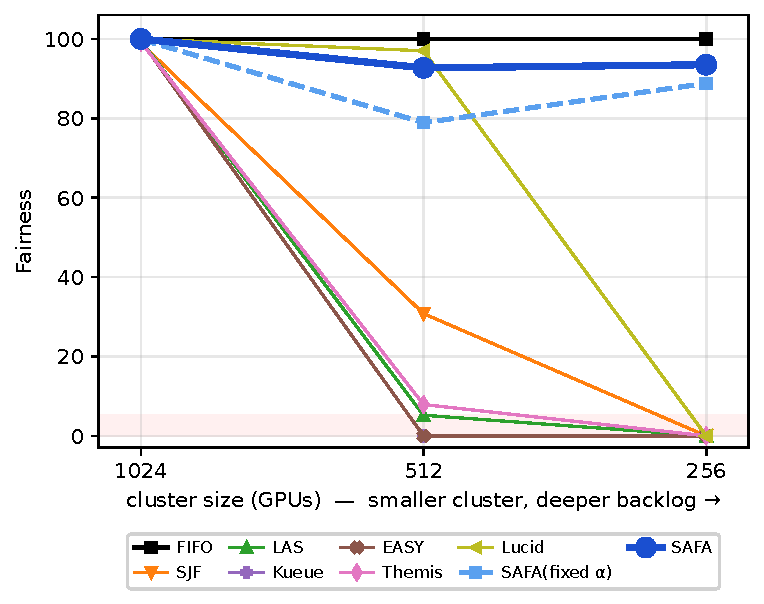
\includegraphics[width=\columnwidth]{Pic/Fig_cliff.pdf}}
\caption{Load--fairness cliff.}
\label{fig:cliff}
\end{figure}



\paragraph{Distributional fairness}
To assess equity across the whole workload, we also examine the distributional fairness of waiting times (single 256). SAFA's Gini of 0.38 is at FIFO's level (0.36) and more equal than most reordering baselines (0.94--0.95), and its TailRatio of 2 contrasts with the explosions of the reordering baselines (SJF 13,336; Themis 3,082; Lucid 2,179). LAS and EASY have low Gini (0.45, 0.40) yet collapse to Fairness 0---distributionally even but order-unfair---showing that both axes must be read together for SAFA's advantage to be seen as more than the artifact of a single measure.

\begin{figure}[htb!]
\centerline{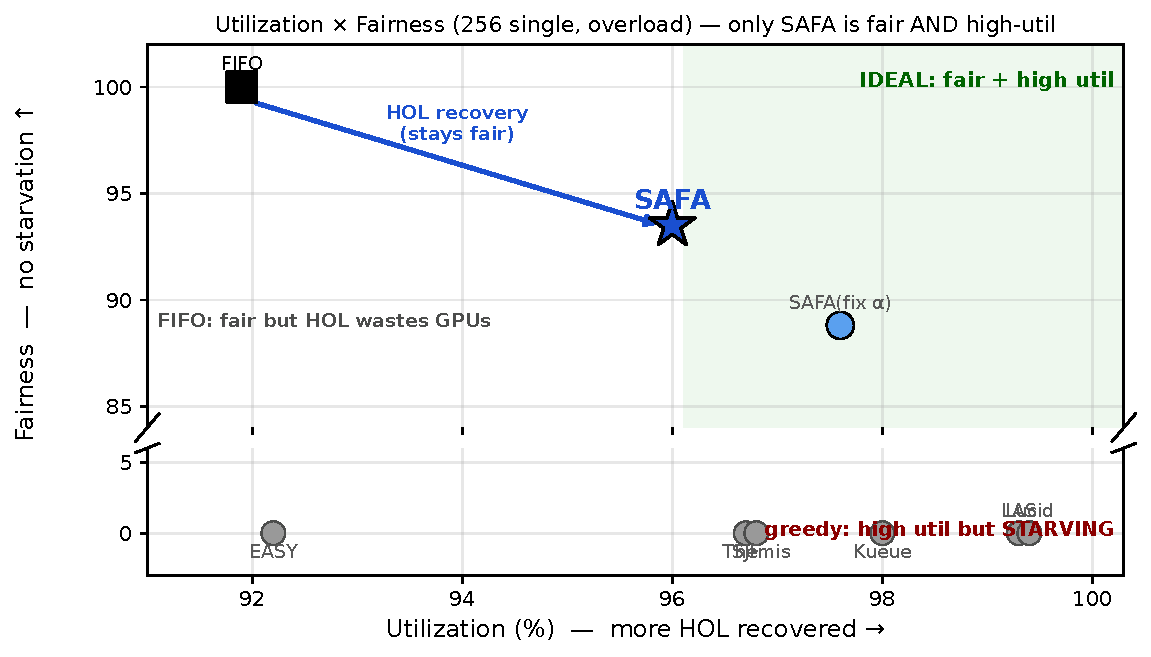
\includegraphics[width=\columnwidth]{Pic/Fig_tradeoff.pdf}}
\caption{Utilization--fairness trade-off.}
\label{fig:tradeoff}
\end{figure}

\begin{table}[htb!]
\centering
\caption{Comparison against grid-searched $\alpha$}
\label{tab:ablation-grid}
\footnotesize
\begin{tabular}{@{}ll@{\hspace{0.8em}}rr@{\hspace{0.8em}}rr@{}}
\toprule
 & & \multicolumn{2}{c}{\textbf{Optimal fixed $\alpha$}} & \multicolumn{2}{c}{\textbf{SAFA (tuning-free)}} \\
\cmidrule(lr){3-4}\cmidrule(lr){5-6}
 & \textbf{GPU} & Fairness\,($\alpha^\ast$) & MedianWait & Fairness & MedianWait \\
\midrule
 & 256  & 88.8\,(0.14) & 4.4M & \textbf{93.5} & 5.0M \\
                     & 512  & 90.6\,(0.9)  & 1.3M & \textbf{92.7} & 1.5M \\
                     & 1024 & 100\,(0.01)  & 2    & 100           & 2    \\
\bottomrule
\end{tabular}
\end{table}

\paragraph{Zero-knob effect}
The Fairness difference between fixed $\alpha$ and Zero-knob can be seen in Tables \ref{tab:sim-single} and \ref{tab:ablation-grid}. Table \ref{tab:ablation-grid} finds the per-configuration optimal fixed $\alpha$ on the same Philly trace via the objective function (Eq. \eqref{eq:09}) and compares it with Zero-knob. The point is not the score gap but the removal of re-tuning---the optimal fixed $\alpha$ itself scatters from 0.01 to 0.9 across configurations and must be re-fit when the workload changes, whereas Zero-knob holds Fairness 94/97.6/99.9 across the three traces without any additional preparation.


\subsection{Generalization to Independent Traces}\label{eval:robust:trace}
The evaluation so far has rested on the single Philly trace. We therefore test whether SAFA's key trends reproduce on other workloads using additional public, independent traces.
We first applied the same evaluation to the Venus cluster trace of the Helios\cite{hu2021helios} (SenseTime, SC'21) datacenter (independent of Philly; 125,303 jobs) (summarized in Table \ref{tab:trace3}; overloaded single 80 GPUs). We used the population of 123,969 jobs, excluding 1{,}334 jobs that exceed the cluster capacity (80 GPUs) and could not be placed by any policy. The results show a trend similar to Philly's. Every reordering baseline collapses to Fairness 0 (Overtaken 6.4--22.8\%) while SAFA holds Fairness 97.6 and Overtaken 0.0 (fixed $\alpha$: 92.5). We then replayed the Alibaba PAI\cite{weng2022mlaas} (NSDI'22) trace (Table \ref{tab:trace3}; a seed-42 16.4\% subsample of 120,105 jobs, load multiplier matched to Philly), and the same trend was again confirmed.

In sum, the same trend repeats across the three independent traces (Table \ref{tab:trace3}). In overloaded single configurations, the reordering baselines' overtaking unfairness (Overtaken) reaches double digits (7--26\%), whereas SAFA does not collapse on any trace, keeps Overtaken at 0.0, and holds Fairness at 94/97.6/99.9.

\begin{table}[htb!]
\centering
\caption{Generalization on independent large-scale traces}
\label{tab:trace3}
\scriptsize
\setlength{\tabcolsep}{4pt}
\begin{tabular}{@{}l@{\hspace{0.6em}}rr@{\hspace{0.9em}}rr@{\hspace{0.9em}}rr@{}}
\toprule
 & \multicolumn{2}{c}{\textbf{Philly}} & \multicolumn{2}{c}{\textbf{Helios}} & \multicolumn{2}{c}{\textbf{Alibaba}} \\
\cmidrule(lr){2-3}\cmidrule(lr){4-5}\cmidrule(lr){6-7}
\textbf{Policy} & Overtaken & Fairness & Overtaken & Fairness & Overtaken & Fairness \\
\midrule
FIFO          & 0.0   & 100  & 0.0  & 100  & 0.0  & 100 \\
SJF           & 5.8   & 0    & 16.1 & 0    & 6.0  & 0 \\
LAS/Kueue     & 7--8  & 0    & 22.8 & 0    & 10.6 & 0 \\
EASY          & 4.4   & 0    & 8.9  & 0    & 13.4 & 0 \\
Themis        & 6.4   & 0    & 15.2 & 0    & 6.6  & 0 \\
Lucid         & 3.4   & 0    & 6.4  & 0    & 5.7  & 0 \\
SAFA (fixed $\alpha$) & 0.0 & 89 & 0.0 & 92.5 & 0.0 & 94.7 \\
\textbf{SAFA} & \textbf{0.0} & \textbf{94} & \textbf{0.0} & \textbf{97.6} & \textbf{0.0} & \textbf{99.9} \\
\bottomrule
\end{tabular}
\end{table}

\subsection{Placement Composability}\label{eval:robust:placement}
Because SAFA operates at the reordering stage, it can be attached in front of Placement policies. For each of the seven Placement policies (most-allocated, compact, round-robin, MCTS, FGD, KAI binpack, KAI spread), we evaluated performance before (FIFO) and after (SAFA) composition (Table \ref{tab:placement}; single 256 overload; the same 7 metrics as in the main results). Without reordering, the more scattering the placement, the more free GPUs disperse across nodes so that an 8-GPU gang cannot find a node on which it fits as a whole; utilization accordingly falls from 91.9\% (most-allocated) to 89.3\% (KAI spread), and the median wait grows from 5.8M\,s to 6.2M\,s --- fragmentation costs are real for every placement, and their size varies.

SAFA improves every metric on all seven Placement policies. Because the reordering policy fills currently vacant node slots with fitting jobs and patches over fragmentation, it restores utilization to 95--96\% on every placement ($+4$\,$\sim$\,$+6$\%p), lowers the median wait by 14--18\%, and keeps order fairness high, with Fairness at 92--94. Crucially, SAFA's utilization recovery is largest on the worst (scattering) placement---on KAI spread it lifts FIFO's 89.3\% to 95.1\% ($+5.8$\%p; Fig. \ref{fig:placehol}). SAFA thus not only composes with any Placement policy but also acts as a complement that recovers whatever utilization a placement loses to fragmentation. Even a simply implemented Placement policy can attain high efficiency at low cost when combined with SAFA.

\begin{figure}[htb!]
\centerline{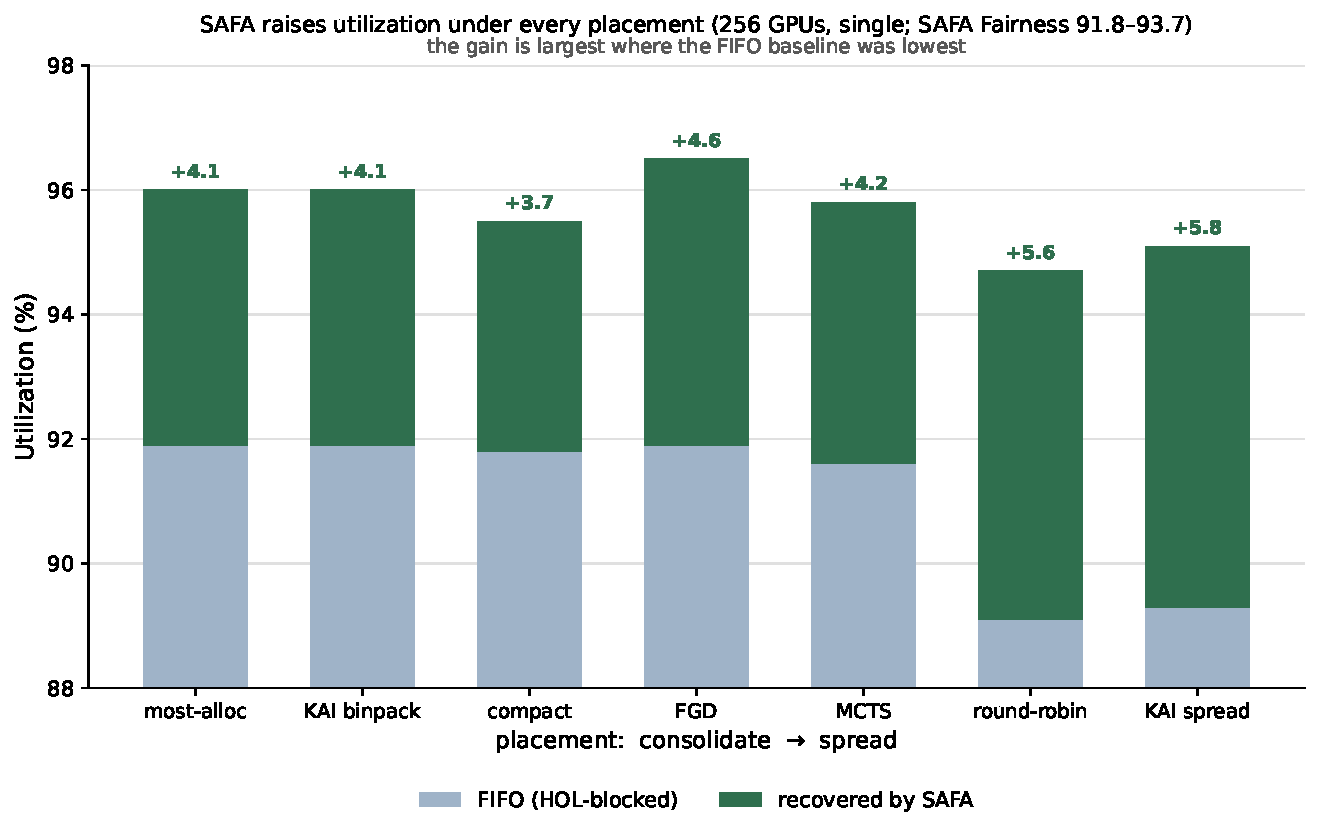
\includegraphics[width=\columnwidth]{Pic/Fig_placement_hol.pdf}}
\caption{HOL recovery by fragmentation.}
\label{fig:placehol}
\end{figure}

\begin{table}[htb!]
\centering
\caption{Metrics before/after composing SAFA with Placements (single 256 overload)}
\label{tab:placement}
\resizebox{\columnwidth}{!}{%
\begin{tabular}{@{}ll rrrrrrr@{}}
\toprule
\textbf{Placement} & & \textit{MedianWait} & \textit{MaxWait} & \textit{Fairness} & Overtaken & \textbf{Utilization} & Gini & TailRatio \\
\midrule
\multirow{2}{*}{most-allocated} & FIFO & 5.8M & 13.0M & 100 & 0.0 & 91.9 & .36 & 2.23 \\
                                & SAFA & 5.0M & 11.9M & 93 & 0.0 & \textbf{96.0} & .38 & 2.36 \\
\multirow{2}{*}{compact}        & FIFO & 5.8M & 13.0M & 100 & 0.0 & 91.8 & .36 & 2.23 \\
                                & SAFA & 5.2M & 12.0M & 93 & 0.0 & \textbf{95.5} & .38 & 2.32 \\
\multirow{2}{*}{round-robin}    & FIFO & 6.1M & 13.8M & 100 & 0.0 & 89.1 & .36 & 2.24 \\
                                & SAFA & 5.1M & 12.4M & 92 & 0.0 & \textbf{94.7} & .39 & 2.42 \\
\multirow{2}{*}{MCTS}           & FIFO & 5.8M & 13.1M & 100 & 0.0 & 91.6 & .36 & 2.24 \\
                                & SAFA & 5.1M & 12.1M & 94 & 0.0 & \textbf{95.8} & .38 & 2.35 \\
\midrule
\multirow{2}{*}{FGD}            & FIFO & 5.8M & 13.1M & 100 & 0.0 & 91.9 & .36 & 2.24 \\
                                & SAFA & 5.0M & 12.0M & 94 & 0.0 & \textbf{96.5} & .38 & 2.37 \\
\multirow{2}{*}{KAI binpack}    & FIFO & 5.8M & 13.0M & 100 & 0.0 & 91.9 & .36 & 2.23 \\
                                & SAFA & 5.0M & 11.9M & 93 & 0.0 & \textbf{96.0} & .38 & 2.36 \\
\multirow{2}{*}{KAI spread}     & FIFO & 6.2M & 13.8M & 100 & 0.0 & 89.3 & .35 & 2.23 \\
                                & SAFA & 5.1M & 12.3M & 92 & 0.0 & \textbf{95.1} & .39 & 2.42 \\
\bottomrule
\end{tabular}}
\end{table}

\subsection{Real-Cluster Validation (B200)}\label{eval:b200}
We cross-validate whether the starvation prevention shown in simulation also holds on the real Kubernetes admission-and-binding path, on an NVIDIA B200$\times$8 single-node cluster (K8s v1.31). The trace is a 500-job Philly sample replayed with only time compressed while preserving the original trace's bursty pattern of clustered submissions --- at the peak, the pending jobs' summed GPU demand is 12$\times$ the capacity (8 GPUs) and up to 440 of the 500 jobs wait simultaneously, forming a deep backlog in which age promotion is actually needed. Each job passed through the kube-scheduler path (creation, gating, binding) as a sleep stub that actually occupies GPUs (6 runs $\times$ 500 jobs $=$ 3{,}000 real Pods including policies and repetitions); we measure the fidelity of the admission-and-binding path and exclude real computation and communication.

The validation shows that the simulator's starvation prevention is reproduced on the real cluster as well. SAFA maintained fairness and prevented starvation under burst overload (Fairness 82.8, Overtaken 0.0\%, deviation $\pm$0.2 across repetitions), while a control run altered to keep dispatching later jobs while ignoring the head's wait collapsed to Fairness 3.8.

On a single node, however, fragmentation and resource-fitness differences cannot extend across nodes, so SAFA's effect appears less pronounced.

\subsection{Limitations}\label{eval:threats}
Even after the three-trace validation and the Placement-composition validation above, the following limitations remain in this evaluation, so the results should be interpreted as trends rather than absolute values.

(1) Measurement/model scope. Real-cluster validation is limited to burst replay on a B200$\times$8 single node (SAFA, FIFO, control run); a measured comparison of all Order policies and end-to-end measurement of multi-node fragmentation are future work. Network and inter-job interference were not modeled, and per-job type--throughput differentials were not examined. Extending $R$ to per-type, node-group, and multi-dimensional resources is a prerequisite task.

(2) Workload/comparison scope. The main evaluation is Philly-based and reinforced with Helios and Alibaba, but all are finite samples, and SOTA (Sia, etc.) was excluded for missing decision variables. Our contribution is limited to ``a pre-placement reordering layer without auxiliary information,'' not ``better than every scheduler.''

(3) BSLD\cite{feitelson1998metrics} can structurally favor short jobs and Fairness can favor arrival-order-preserving policies, so we cross-checked with independent distributional metrics (Gini, TailRatio, Overtaken in Table \ref{tab:sim-single}) (the advantage holds under overload). The main results table does not include per-cell comparisons against reference values, but the headline contrast (reordering baselines' Fairness$\approx$0 vs. SAFA's 92--95) is an order-of-magnitude difference and thus robust.

Overall, our conclusion asserts no absolute ranking; instead, it emphasizes the fairness-collapse-versus-utilization trade-off that emerges as load deepens.

\FloatBarrier

\section{CONCLUSIONS AND FUTURE WORKS}\label{conclu}

This work proposed SAFA, which handles Order alone --- the first stage of scheduling --- to resolve HOL-blocking starvation in GPU server pools. The evaluation was carried out with a discrete-event simulator replaying three traces (Philly, Helios, Alibaba PAI) (on 256--1024-GPU single clusters, comparing against FIFO and six Order policies and validating composition with seven Placements) and with real measurements on NVIDIA B200$\times$8 Kubernetes (cross-validation). Unlike a variety of recent scheduler policies that require runtime estimation, performance profiles, or solvers, SAFA resolves queue-head HOL with queue-observable information only (waiting time, resource demand, relative age) and operates on top of a range of schedulers.

SAFA (Zero-knob) preserves fairness while also leading on efficiency. In the deepest overload, while the Fairness of all six Order policies collapses to 0, SAFA holds 92--95, cuts the median wait by 7--13\% relative to FIFO, and raises utilization from 92\% to 95--96\%; the same picture repeats on the independent traces (Helios, Alibaba). Under light, low-contention conditions, collocation policies like Lucid can be faster and fairer, but as load deepens, reordering policies suffer order-fairness collapse and size-selective policies starve large jobs. SAFA was the only balance point restraining both axes with queue-observable information alone.

A fixed $\alpha$ required repeated search for its optimum, and that value varied greatly with workload characteristics. SAFA therefore introduces Zero-knob, which needs no tuning and adapts to workload changes using only observed queue statistics (relative age, resource fitness $R$).

Since this work is limited to GPU gang traces (Philly, Helios, Alibaba), extending the evaluation to classical parallel-job traces in the Standard Workload Format (SWF) to bridge to the classical HPC batch-scheduling literature also remains future work.

The B200 measurements confirmed that on the real Kubernetes admission-and-binding path SAFA prevents burst-overload starvation (Fairness 82.8, Overtaken 0.0\%) and that the decisive factor is head-order preservation. The multi-node, fragmented conditions do not form on a single node, so the most important future work is expanding the real-cluster measurements.

\FloatBarrier
\section*{ACKNOWLEDGMENT}
The authors received no financial support from any institution for this work.

Disclosure of generative-AI use. Following IEEE recommendations, the authors disclose that generative-AI tools were used in an auxiliary capacity in preparing this paper. AI was used only for sentence polishing and language editing, figure generation and scripts for reproducing experiments, and assistance in organizing results; the conception of the research, algorithm design, and the execution and interpretation of experiments were carried out by the authors themselves. The authors reviewed and revised all content after using AI tools and bear full responsibility for the content of the publication.

\bibliographystyle{IEEEtran}
\bibliography{sn-bibliography}
%% if required, the content of .bbl file can be included here once bbl is generated
%%\input sn-article.bbl

% Author biographies --- to add a photo, replace IEEEbiographynophoto with
% \begin{IEEEbiography}[{\includegraphics[width=1in,height=1.25in,clip,keepaspectratio]{photo}}]{Name}.
% Fill in the XXXX/XX placeholders with actual degrees and years.
\begin{IEEEbiography}[{
\includegraphics[width=1in,height=1.25in,clip,keepaspectratio]{Pic/bio_kyunam_cho.jpg}}]{Kyunam Cho}~is a Research Fellow at LG Uplus in Seoul and is also a Ph.D. candidate in computer science at Korea University in Seoul, Korea. From 2000 to 2021, he worked as a software developer and software architect at Samsung Electronics. From 2021 to 2022, he worked as a software architect at Hyundai Card Company.

His main research area is high-performance computing (HPC) and HPC-applied software platforms. He has built and operated thousands of GPGPU-based machine learning systems at Samsung Electronics. Currently, his interests include large language model ops known as LLMOps, federated learning, and chaos engineering for public cloud-based platforms. He authored a book on machine learning and has published papers in Computer Physics Communications.

\end{IEEEbiography}

\begin{IEEEbiography}[{
\includegraphics[width=1in,height=1.25in,clip,keepaspectratio]{Pic/bio_younghwan_jin.jpg}}]{YoungHwan Jin}~received the B.S. degree in XX from XX University in XXXX. He currently works at LG Uplus Corp., Seoul, Republic of Korea. His research interests include GPU cluster operations, datacenter infrastructure, and cloud computing.
\end{IEEEbiography}

\begin{IEEEbiography}[{
\includegraphics[width=1in,height=1.25in,clip,keepaspectratio]{Pic/bio_heonchang_yu.jpg}}]{Heonchang Yu}~is a Professor with the Department of Computer Science and Engineering, Korea University, Seoul, Korea. He received the M.S. and Ph.D. degrees in computer science from Korea University in 1991 and 1994, respectively. He has been a Professor at Korea University since 1998, and was a Visiting Professor with the Department of Electrical and Computer Engineering, University of Texas at San Antonio, TX, USA, from 2019 to 2020. He leads the Distributed and Cloud Computing Laboratory at Korea University.

His research interests include cloud computing, virtualization (including GPU virtualization), distributed systems, fault-tolerant systems, and edge cloud technology supporting real-time processing. He has served as an editor of the Korean Institute of Information Scientists and Engineers since 2007.
\end{IEEEbiography}

\end{document}
